\section{Results}
Smoke results are generated by \texttt{make smoke}. The MVP reports local heuristic and spec-first baselines on the development split, with figures saved under \texttt{paper/figures/}.

\begin{table}[h]
\centering
\begin{tabular}{llllll}
\toprule
Suite & Agent & Model & CC-F1 & Task success & Near-miss detection \\
\midrule
Smoke & Heuristic & Mock & see \texttt{paper/tables/main\_results.csv} & see CSV & see CSV \\
Smoke & Spec-first & Mock & see \texttt{paper/tables/main\_results.csv} & see CSV & see CSV \\
Full API & Direct & TBD & Placeholder & Placeholder & Placeholder \\
Full API & Plan-first & TBD & Placeholder & Placeholder & Placeholder \\
Full API & Spec-first & TBD & Placeholder & Placeholder & Placeholder \\
Full API & Oracle-spec & TBD & Placeholder & Placeholder & Placeholder \\
\bottomrule
\end{tabular}
\caption{Main results table template. Replace placeholders with audited API-backed aggregates before submission.}
\end{table}

\begin{table}[h]
\centering
\begin{tabular}{lllll}
\toprule
Domain & Agent & CC-F1 & Task success & Near-miss detection \\
\midrule
Calendar & TBD & Placeholder & Placeholder & Placeholder \\
Email & TBD & Placeholder & Placeholder & Placeholder \\
Sheet/database & TBD & Placeholder & Placeholder & Placeholder \\
CRM/workflow & TBD & Placeholder & Placeholder & Placeholder \\
File/document & TBD & Placeholder & Placeholder & Placeholder \\
\bottomrule
\end{tabular}
\caption{Domain-stratified results template. The smoke aggregate is exported to \texttt{results/by\_domain.csv}.}
\end{table}

\begin{figure}[h]
\centering
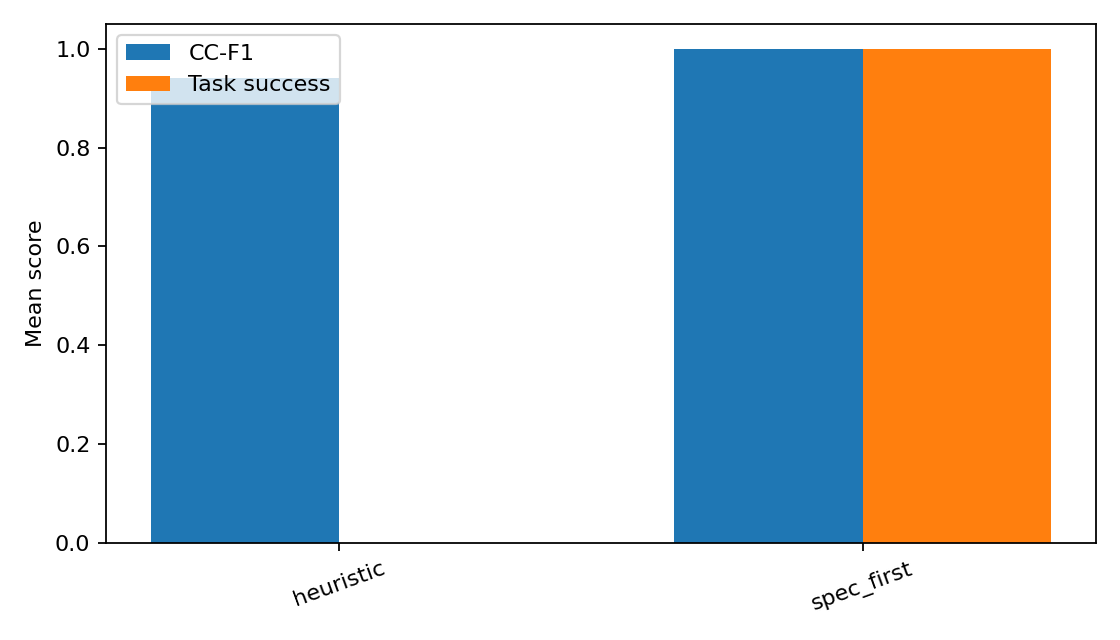
\includegraphics[width=0.8\linewidth]{figures/main_results_by_agent.png}
\caption{Results by agent.}
\end{figure}

\begin{figure}[h]
\centering
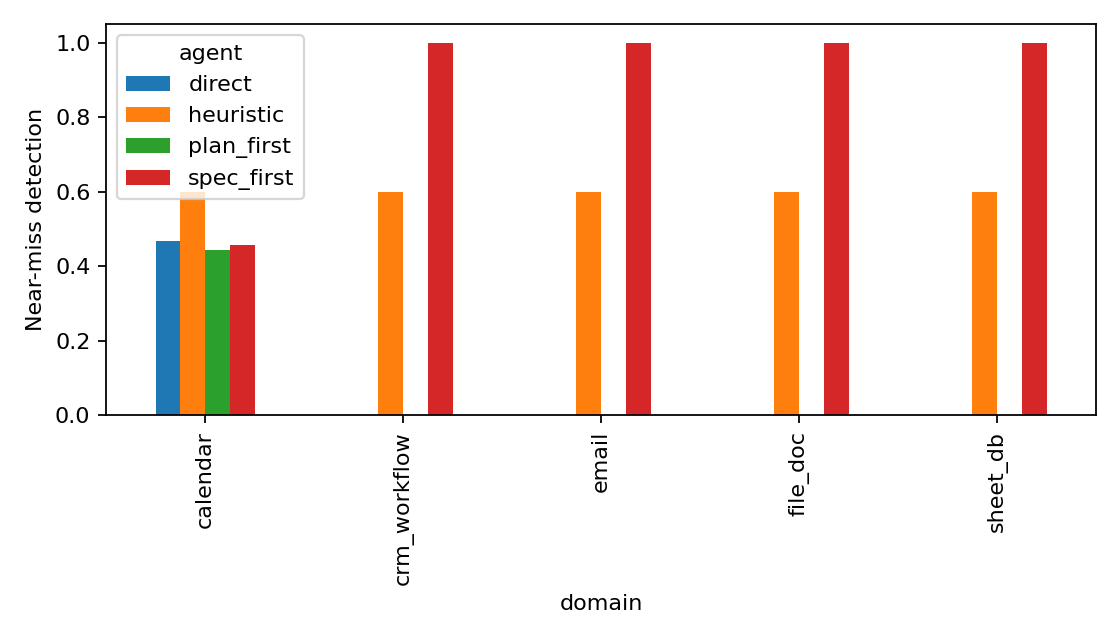
\includegraphics[width=0.8\linewidth]{figures/near_miss_by_domain.png}
\caption{Near-miss mutation examples and detection by domain.}
\end{figure}
